% Special title page command to get a different background
\begin{frame}
    \titlepage
\end{frame}

\section{Oppgaver}

\begin{frame}{Innholdsfortegnelse}

\begin{itemize}
    \item Introduksjon
    \item Nyttige tips før eksamen
    \item Nyttige tips under eksamen
    \item Oppgaveregning
\end{itemize}Q
    
\end{frame}

\begin{frame}
    \frametitle{Før eksamen}
    \begin{itemize}
        \item For forståelsen: \url{http://mathinsight.org/thread/multivar}
        \item Matte 2: Oppgaveløsning på video. \url{https://video.adm.ntnu.no/serier/52f0b7e0294b4}
        \item Lag en frekvenstabell over tidligere gitte eksamensoppgaver
        \item Øv til eksamen mest mulig likt eksamen. Ta tiden, bruk LF sparsomt. 
        \item Matte 2 eksamener er $99\%$ likt Ma1103, regn de og!
    \end{itemize}
\end{frame}

\begin{frame}
  \frametitle{Før eksamen}
  \begin{enumerate}
    \item \textbf{Alltid} ny deloppgave på ny side
    \item Tegn store figurer 
    \item Stor frokost + rask mat under eksamen
    \item Slapp av! Selv om eksamen ikke går helt som planlagt har du fortsatt Delta. 
  \end{enumerate}
\end{frame}


\begin{frame}
  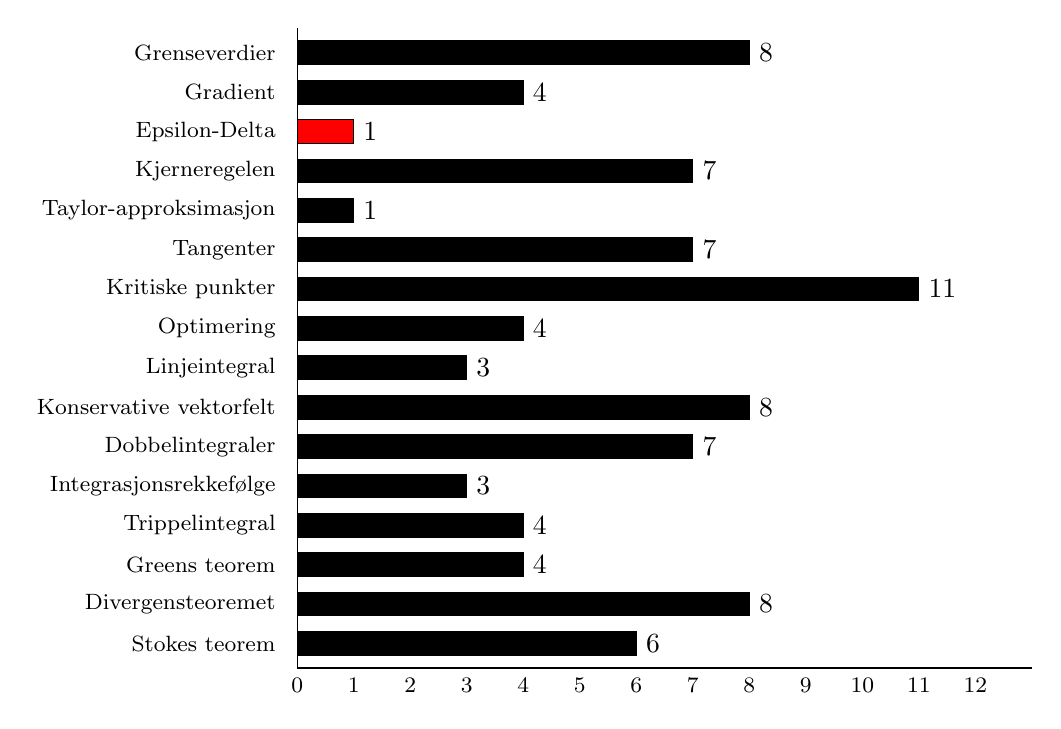
\begin{tikzpicture}
    \begin{axis}[ xbar=0pt, /pgf/bar shift=0pt, legend style={ legend columns=4,
        at={(xticklabel cs:0.5)}, anchor=north, draw=none }, ytick={0,...,15},
      ytick style={draw=none},% <- added
      axis y line*=none, axis x line*=bottom, tick label
      style={font=\footnotesize}, legend style={font=\footnotesize}, label
      style={font=\footnotesize}, xtick style={draw=none},% <- added
      xtick={0,1,...,12}, width=.9\textwidth, bar width=3mm, y dir = reverse,
      yticklabels={%
        {Grenseverdier}, {Gradient}, {Epsilon-Delta}, {Kjerneregelen},
        {Taylor-approksimasjon}, {Tangenter}, {Kritiske punkter}, {Optimering},
        {Linjeintegral}, {Konservative vektorfelt}, {Dobbelintegraler},
        {Integrasjonsrekkefølge}, {Trippelintegral}, {Greens teorem},
        {Divergensteoremet}, {Stokes teorem}}, xmin=0, xmax=13, area legend,
      y=5mm, enlarge y limits={abs=0.625}, nodes near coords, nodes near coords
      style={text=black}, every axis plot/.append style={fill} ]
      \addplot[fill=black] coordinates {(8,0)}; \addplot[fill=black] coordinates
      {(4,1)}; \addplot[fill=red] coordinates {(1,2)}; \addplot[fill=black]
      coordinates {(7,3)}; \addplot[fill=black] coordinates {(1,4)};
      \addplot[fill=black] coordinates {(7,5)}; \addplot[fill=black] coordinates
      {(11,6)}; \addplot[fill=black] coordinates {(4,7)}; \addplot[fill=black]
      coordinates {(3,8)}; \addplot[fill=black] coordinates {(8,9)};
      \addplot[fill=black] coordinates {(7,10)}; \addplot[fill=black]
      coordinates {(3,11)}; \addplot[fill=black] coordinates {(4,12)};
      \addplot[fill=black] coordinates {(4,13)}; \addplot[fill=black]
      coordinates {(8,14)}; \addplot[fill=black] coordinates {(6,15)};
    \end{axis}
  \end{tikzpicture}
\end{frame}

%%% Local Variables:
%%% mode: latex
%%% TeX-master: "main"
%%% End:
